\chapter{Analytická část}\label{chap:anal}

V této kapitole se budu věnovat analýze aktuálního stavu testovací knihovny a možnostech jejího rozšíření.


\section{Analýza stávajícího stavu knihovny}

Původní testovací knihovna byla výstupem mojí bakalářské práce\cite{bakalarka} dokončené v roce 2021. Cílem této knihovny byla automatizace testů verifikace průmyslové komunikace a integrace do kontinuálního testování na Azure DevOps serveru. 

Knihovna rozlišuje tři druhy účastníků testování:

\begin{description}
    \item[Testovací služba] Služba, která řídí testovací běh.
    \item[Testované zařízení] Hlavní účastník testování, který běží na jiném zařízení, než ze kterého běží testovací služba. 
    \item[Testovací partner] Zařízení, které simuluje nějaké testované zařízení. Toto zařízení běží na stejném zařízení, jako testovací služba. 
\end{description}

Ideou knihovny je, že testovací služba, která řídí a synchronizuje běh na všech zúčastněných zařízení, je spouštěna automatizovaně za pomoci Azure DevOps serveru v Azure Pipelines. Společně s ním je spuštěn i vyvíjený produkt, který chceme otestovat, v tomto kontextu nazýván jako testované zařízení. Testované zařízení se následně připojí k testovací službě a po úspěchu této fáze započne samotné testování. 

Pro každý test lze definovat další účastníky testování - testovací partnery. Tito testovací partneři běží pouze po dobu daného testu a po dokončení testu zaniknou. Hlavní úlohou těchto zařízení je simulace protistrany při komunikaci. 

Ukázka možného propojení všech účastníků testování můžeme vidět na obrázku \ref{fig:bp_devicemodel}. Jak zde je vidět, testovací partneři a testovací služba běží na jednom zařízení, takzvaném agentovi, na kterém je primárně spouštěno celé testování. Vlevo dole je vidět testované zařízení SIMATIC ET 200SP, které je propojeno s agentem. Vpravo dole můžeme vidět PLC, které pouze znázorňuje možnost propojení s dalšími externími zařízeními.

\begin{figure}[htbp]
    \centering 
    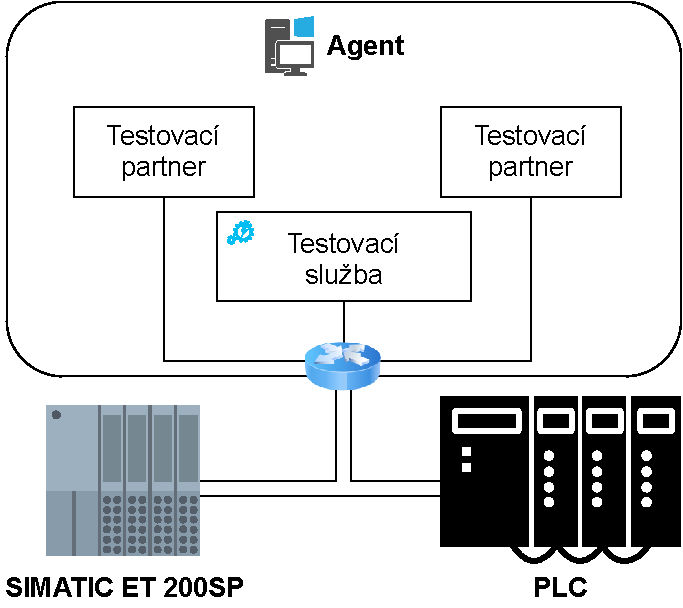
\includegraphics[width=0.97\textwidth]{assets/img/bp_assets/devicemodel.pdf}
    \caption{Ukázka možného propojení účastníků testování v původní knihovně}
    \source{\cite{bakalarka}}
    \label{fig:bp_devicemodel}
\end{figure}

